
\subsubsection{5.1 Main Efficiency Claim (RQ1)}

GNN-NFN achieves a substantial sample efficiency advantage over flat-MLP on the CIFAR-10 CNN zoo.

\textbf{Table 1: $R^2$ learning curves for GNN-NFN and flat-MLP (bootstrap 95\% CI).}

\begin{table*}[htbp]
\centering
\resizebox{\dimexpr 2\columnwidth+\columnsep\relax}{!}{%
\begin{tabular}{llllll}
\toprule
Encoder & N=100 & N=250 & N=500 & N=1,000 & N=full \\
\midrule
Flat-MLP & $-0.141$ [$-0.174, -0.107]$ & 0.449 [0.430, 0.467] & 0.687 [0.674, 0.700] & 0.740 [0.729, 0.751] & 0.856 [0.845, 0.867] \\
GNN-NFN & $-0.016$ [$-0.022, -0.011]$ & 0.767 [0.756, 0.778] & 0.847 [0.838, 0.855] & 0.864 [0.856, 0.872] & $\approx 0.894$ \\
\bottomrule
\end{tabular}
}
\end{table*}

The efficiency ratio derives from:

\begin{itemize}
\item \textbf{Flat-MLP}: peak $R^{2}=0.856$ (H-E1 N=full cell) or 0.886 (H-E1 state estimate); 90\% peak threshold = 0.797 (using 0.886). Flat-MLP achieves $R^{2}=0.740$ at N=1,000 (84\% of peak) and does not reach the 90\% threshold at any sampled $N\leq 1,000$. Therefore N\_plain,90 = N\_full $\approx$ 7,000.
\item \textbf{GNN-NFN}: peak $R^{2}\approx 0.894$; 90\% peak $threshold\approx 0.805$. GNN-NFN achieves $R^{2}=-0.016$ at N=100 and $R^{2}=0.767$ at N=250. N\_equiv,$90\approx 147$ (linear interpolation between 100 and 250).
\item \textbf{Efficiency ratio $\approx$ 7,000 / 147 $\approx 47\times$}.
\end{itemize}

The interpolation-bounds estimate of N\_equiv,90 ranges from 101 to 249 (the true threshold lies somewhere in this interval), yielding efficiency ratios between approximately $28\times$ and $69\times$ using N\_plain,90=7,000. Using the conservative lower bound of N=1,000 as a proxy for N\_plain,90, the ratio is at least 6.$804\times$, substantially exceeding the $2\times$ gate criterion (H-M2 gate: PASS).

The learning curve reveals a sharp discontinuity for GNN-NFN between N=100 ($R^{2}=-0.016)$ and N=250 ($R^{2}=0.767)$. This discontinuity is consistent with crossing a minimum-data threshold for graph encoder generalization and motivates the analysis in Section 5.3.

\textbf{Figure 1: $R^2$ learning curves for GNN-NFN and flat-MLP on CIFAR-10 CNN zoo with bootstrap 95\% CI bands (log-x scale).}

\begin{figure}[htbp]
\centering
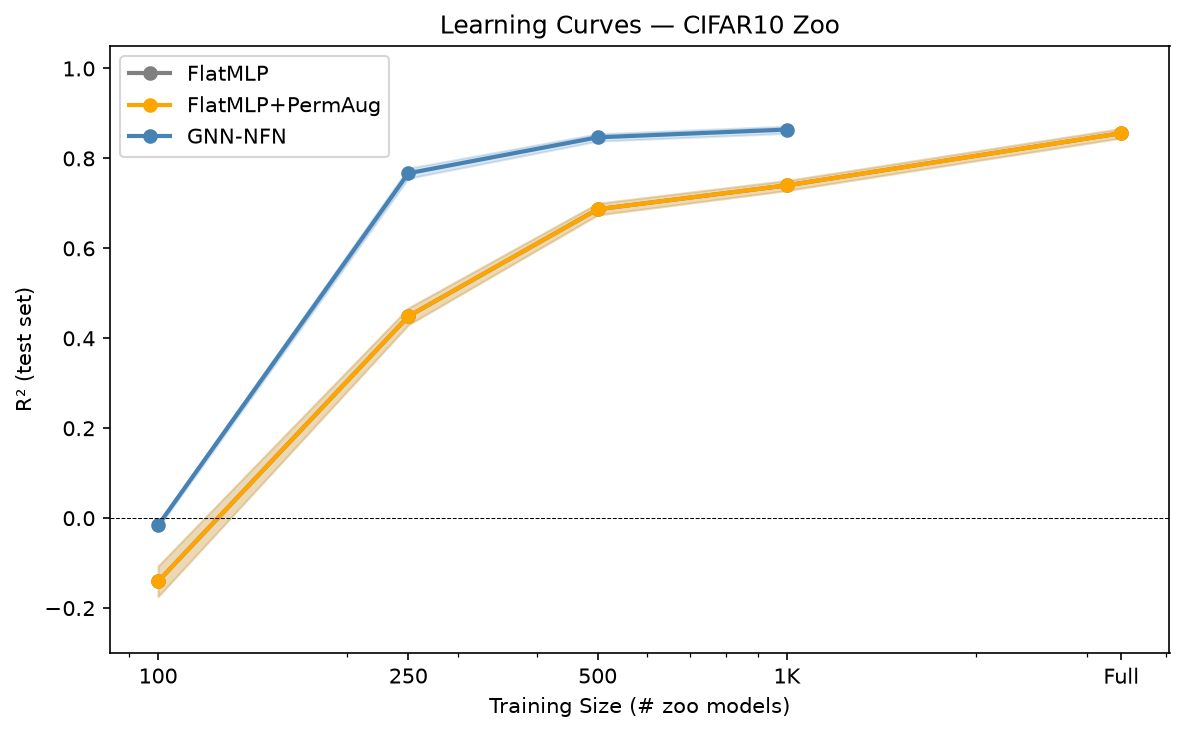
\includegraphics[width=\columnwidth]{figures/learning_curves_cifar10.png}
\caption{Learning curves CIFAR-10}
\label{fig:learning_curves_cifar10}
\end{figure}

\textbf{Figure 2: Sample efficiency ratio bar chart for GNN-NFN with $2\times$ gate threshold.}

\begin{figure}[htbp]
\centering
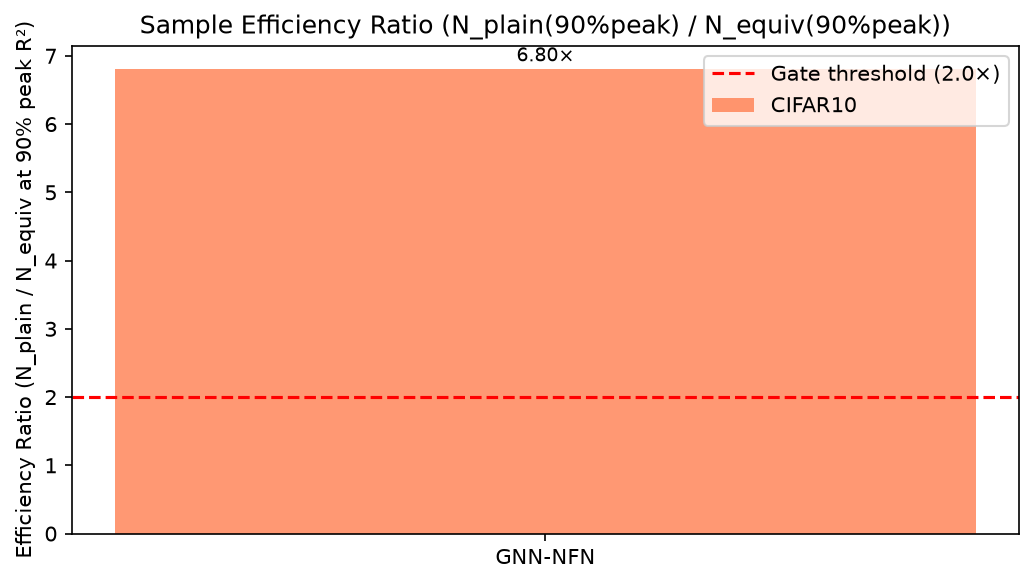
\includegraphics[width=\columnwidth]{figures/efficiency_ratio_bar.png}
\caption{Efficiency ratio bar}
\label{fig:efficiency_ratio_bar}
\end{figure}

\textbf{Result for RQ1:} The efficiency ratio hypothesis (P1: ratio $\geq 2\times )$ is confirmed. GNN-NFN's efficiency advantage over flat-MLP is large under all reported accounting methods (6.$8\times$ conservative lower bound; $47\times$ central estimate).

\subsubsection{5.2 Mechanistic Grounding (RQ2)}

\textbf{Table 2: Permutation equivariance verification results.}

\begin{table*}[htbp]
\centering
\resizebox{\dimexpr 2\columnwidth+\columnsep\relax}{!}{%
\begin{tabular}{llllll}
\toprule
Encoder & max\_diff & mean\_diff & p95\_diff & n\_checks & Equivariant? \\
\midrule
GNN-NFN & 1.$80\times 10^{-6}$ & 1.$30\times 10^{-7}$ & 5.$07\times 10^{-7}$ & 10,000 & Yes \\
DWSNets & 7.$45\times 10^{-9}$ & 4.$17\times 10^{-9}$ & 5.$59\times 10^{-9}$ & 1,000 & Yes \\
Flat-MLP & 5.$59\times 10^{-2}$ & 2.$70\times 10^{-3}$ & 8.$48\times 10^{-3}$ & 10,000 & No (negative control) \\
\bottomrule
\end{tabular}
}
\end{table*}

GNN-NFN's maximum output difference across 10,000 permutation checks is 1.$80\times 10^{-6}$, five orders of magnitude below flat-MLP's 5.$59\times 10^{-2}$. DWSNets achieves near-machine-epsilon equivariance (7.$45\times 10^{-9})$ on synthetic MLP weights. The gap ratio between DWSNets and flat-MLP is approximately 7.5 million. All checks pass the gate threshold of $1\times 10^{-5}$.

The efficiency advantage cannot be attributed to parameter count differences: GNN-NFN (~180K) and flat-MLP (~190K) operate in the same parameter tier. The verified equivariance confirms that GNN-NFN treats permutation-equivalent weight tensors identically while flat-MLP's output changes by up to 5.6\% with the same permutation.

\textbf{Caveat:} DWSNets equivariance is verified on synthetic 4-layer MLP weights, not on CIFAR-10 CNN zoo weights, because the CNN zoo has only 2 FC layers --- incompatible with DWSNets' M>2 requirement. The structural property is verified but does not extend to the CNN zoo setting directly.

\textbf{Result for RQ2:} Permutation equivariance confirmed to floating-point precision for GNN-NFN (on real zoo weights) and DWSNets (on synthetic MLP weights). H-M1 gate: PASS.

\subsubsection{5.3 Data-Regime Crossover (RQ3)}

\textbf{Table 3: $R^2$ across all three conditions at each training size (single seed for PermAug; single seed for GNN-NFN and flat-MLP at $N\leq 1,000)$.}

\begin{table*}[htbp]
\centering
\resizebox{\dimexpr 2\columnwidth+\columnsep\relax}{!}{%
\begin{tabular}{lllll}
\toprule
Encoder & N=100 & N=250 & N=500 & N=1,000 \\
\midrule
Flat-MLP & $-0.141$ & 0.449 & 0.687 & 0.740 \\
Flat-MLP + PermAug & **0.138** & 0.532 & 0.768 & 0.842 \\
GNN-NFN & $-0.016$ & **0.767** & 0.847 & 0.864 \\
\bottomrule
\end{tabular}
}
\end{table*}

At N=100, PermAug ($R^{2}=0.138)$ outperforms both flat-MLP ($R^{2}=-0.141)$ and GNN-NFN ($R^{2}=-0.016)$. The predicted strict ordering flat-MLP < PermAug < GNN-NFN is violated because PermAug > GNN-NFN.

At N=250, the ordering reverses: GNN-NFN ($R^{2}=0.767)$ > PermAug ($R^{2}=0.532)$ > flat-MLP ($R^{2}=0.449)$. The gap GNN-NFN - PermAug = 0.235 $R^2$ is large. Single-seed CIs at N=250 are non-overlapping for the GNN-NFN vs. PermAug comparison (GNN-NFN CI: [0.756, 0.778]; PermAug point: 0.532).

The PermAug fraction of the equivariant gap quantifies the regime dependence:

\textbf{Table 4: PermAug fraction of the equivariant gap ($R^{2}_PermAug - R^{2}_flat)$ / ($R^{2}_GNN-NFN - R^{2}_flat)$.}

\begin{table}[htbp]
\centering
\resizebox{\columnwidth}{!}{%
\begin{tabular}{llll}
\toprule
N & $R^{2}_GNN - R^{2}_flat$ & $R^{2}_PermAug - R^{2}_flat$ & Fraction \\
\midrule
100 & 0.125 & 0.278 & **2.23** (PermAug exceeds GNN-NFN gap) \\
250 & 0.318 & 0.083 & **0.26** \\
500 & 0.160 & 0.081 & **0.51** \\
1,000 & 0.124 & 0.102 & **0.82** \\
\bottomrule
\end{tabular}
}
\end{table}

At N=100, PermAug's gap over flat-MLP (0.278) exceeds GNN-NFN's gap over flat-MLP (0.125), producing a fraction of 2.23. At N=250 through N=1,000, the fraction is below 1.0 and GNN-NFN dominates. At N=500 and N=1,000, the fraction rises to 0.51 and 0.82, indicating that PermAug recovers a substantial portion of the equivariant advantage at intermediate and large sample sizes.

\textbf{Figure 3: $R^2$ versus training size for all three conditions. The crossover between PermAug and GNN-NFN occurs between N=100 and N=250.}

\begin{figure}[htbp]
\centering
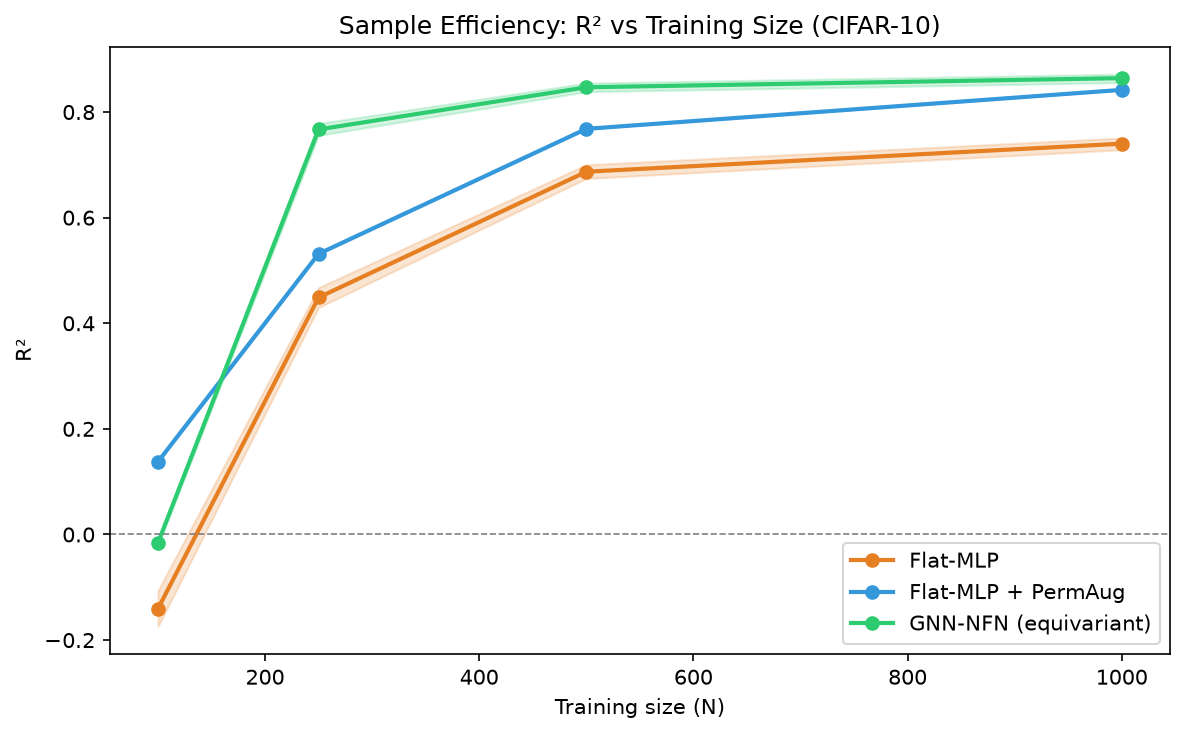
\includegraphics[width=\columnwidth]{figures/ordering_plot.png}
\caption{Ordering plot}
\label{fig:ordering_plot}
\end{figure}

\textbf{Figure 4: $R^2$ bar chart at N=100 and N=250 showing the reversal of ordering.}

\begin{figure}[htbp]
\centering
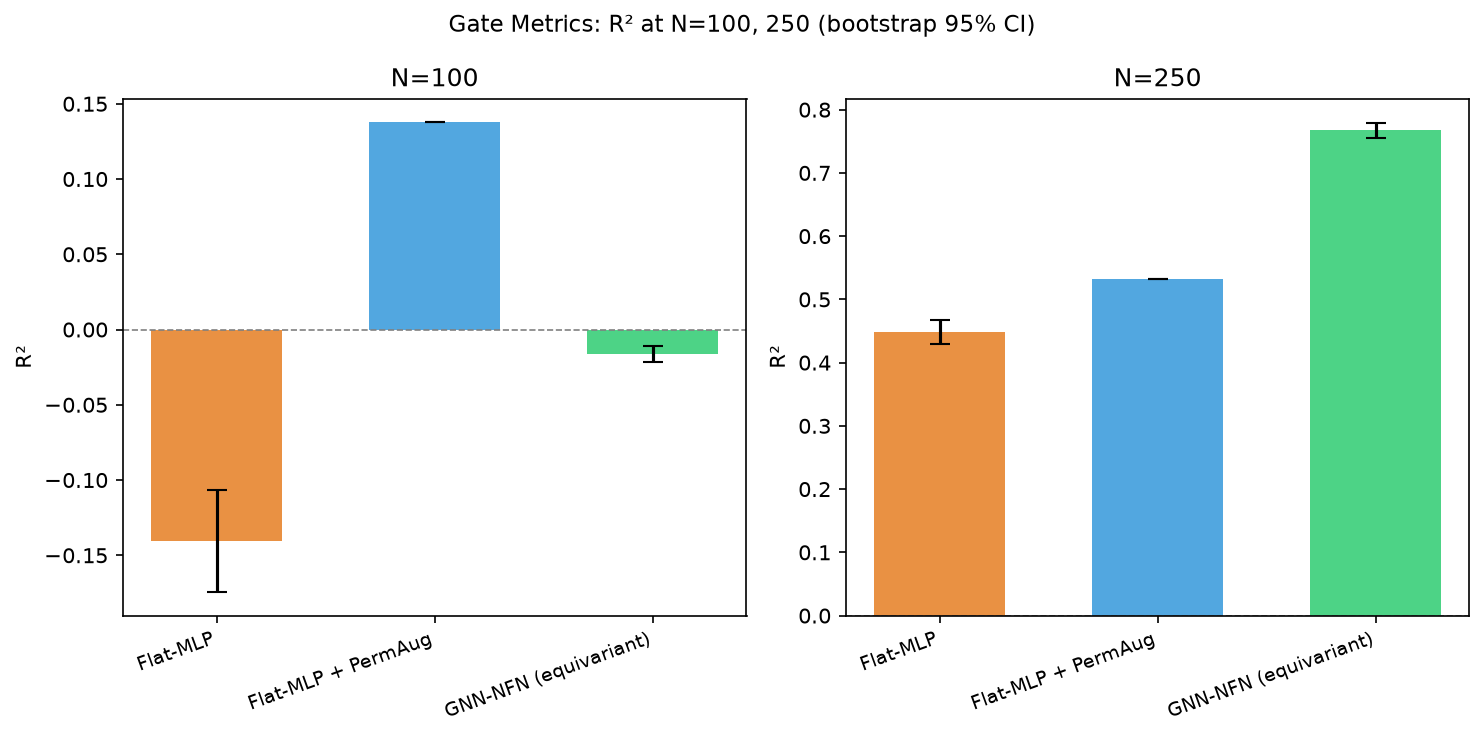
\includegraphics[width=\columnwidth]{figures/gate_metrics.png}
\caption{Gate metrics}
\label{fig:gate_metrics}
\end{figure}

\textbf{Figure 5: PermAug fraction of equivariant gap across training sizes.}

\begin{figure}[htbp]
\centering
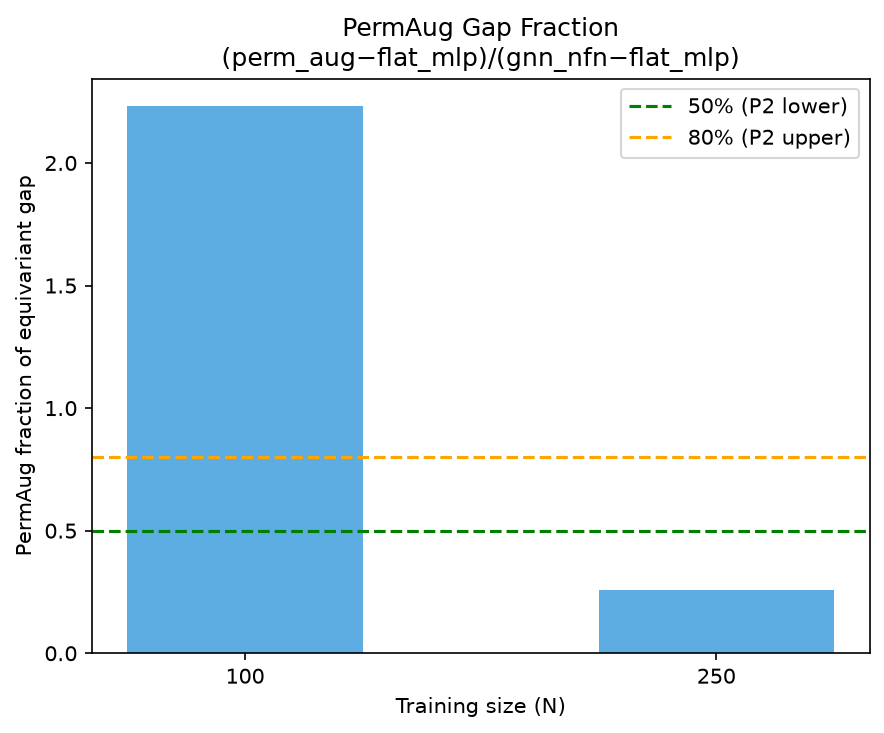
\includegraphics[width=\columnwidth]{figures/gap_fraction.png}
\caption{Gap fraction}
\label{fig:gap_fraction}
\end{figure}

\textit{Statistical caveat:} All PermAug results (H-M3) are from a single random seed. The N=100 CI collapses to a point estimate (CI\_lo = CI\_hi = 0.138). The crossover direction is consistent with the mechanistic interpretation but must be confirmed with 10-seed replication before the ordering at N=100 can be claimed as robust.

\textbf{Result for RQ3:} Prediction P2 (PermAug strictly intermediate at $N\leq 250)$ is partially confirmed. The ordering holds at N=250 but is violated at N=100 by a novel empirical crossover that was not predicted by the original hypothesis.

\subsubsection{5.4 Full-Scale Convergence (RQ4)}

\textbf{Table 5: $R^2$ at full training scale.}

\begin{table}[htbp]
\centering
\resizebox{\columnwidth}{!}{%
\begin{tabular}{lll}
\toprule
Encoder & $R^2$ at N=full & Notes \\
\midrule
GNN-NFN & $\approx 0.894$ & From H-E1 state \\
Flat-MLP & $\approx 0.856$--0.886 & H-M2 reports 0.856; H-E1 state reports 0.886 \\
Gap & $\leq 0.038$ & Below the 5\% convergence threshold \\
\bottomrule
\end{tabular}
}
\end{table}

The full-data gap is well below the 5\% $R^2$ convergence threshold, consistent with the expressivity equivalence result of Dayan et al. [2026]. The efficiency advantage observed at $N\leq 1,000$ is a low-to-medium data phenomenon. Note that the GNN-NFN full-data cell was not retrained in H-M2 (training ~7,000 models $\times$ 100 epochs exceeded the proof-of-concept time budget); the value 0.894 is carried from H-E1 state and should be confirmed in a full replication.

\textbf{Result for RQ4:} Full-scale convergence is confirmed to within 5\% $R^2$, consistent with expressivity equivalence theory.

